\begin{appendices}

\chapter{Graph classes hierarchy}

\begin{figure}
\centering
% Graphic for TeX using PGF
% Title: /home/abde/Documents/memo1819-final/final/scripts/graph_classes.dia
% Creator: Dia v0.97.3
% CreationDate: Mon Feb 11 21:05:39 2019
% For: abde
% \usepackage{tikz}
% The following commands are not supported in PSTricks at present
% We define them conditionally, so when they are implemented,
% this pgf file will use them.
\ifx\du\undefined
  \newlength{\du}
\fi
\setlength{\du}{15\unitlength}
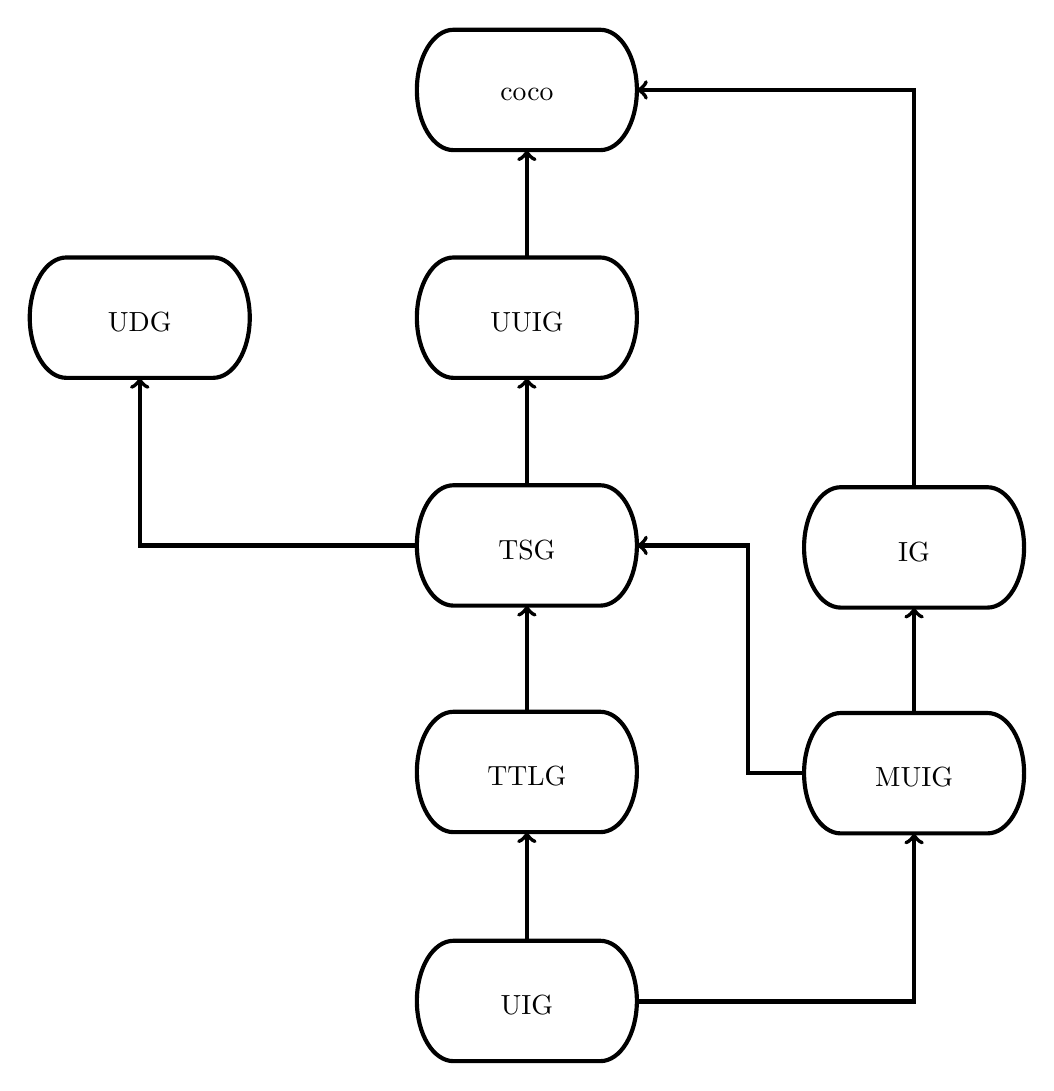
\begin{tikzpicture}
\pgftransformxscale{1.000000}
\pgftransformyscale{-1.000000}
\definecolor{dialinecolor}{rgb}{0.000000, 0.000000, 0.000000}
\pgfsetstrokecolor{dialinecolor}
\definecolor{dialinecolor}{rgb}{1.000000, 1.000000, 1.000000}
\pgfsetfillcolor{dialinecolor}
\pgfsetlinewidth{0.100000\du}
\pgfsetdash{}{0pt}
\pgfsetdash{}{0pt}
\pgfsetbuttcap
\pgfsetmiterjoin
\pgfsetlinewidth{0.100000\du}
\pgfsetbuttcap
\pgfsetmiterjoin
\pgfsetdash{}{0pt}
\definecolor{dialinecolor}{rgb}{1.000000, 1.000000, 1.000000}
\pgfsetfillcolor{dialinecolor}
\pgfpathmoveto{\pgfpoint{17.144160\du}{8.395841\du}}
\pgfpathlineto{\pgfpoint{13.610827\du}{8.395841\du}}
\pgfpathcurveto{\pgfpoint{13.122975\du}{8.395841\du}}{\pgfpoint{12.727493\du}{7.746654\du}}{\pgfpoint{12.727493\du}{6.945841\du}}
\pgfpathcurveto{\pgfpoint{12.727493\du}{6.145027\du}}{\pgfpoint{13.122975\du}{5.495841\du}}{\pgfpoint{13.610827\du}{5.495841\du}}
\pgfpathlineto{\pgfpoint{17.144160\du}{5.495841\du}}
\pgfpathcurveto{\pgfpoint{17.632012\du}{5.495841\du}}{\pgfpoint{18.027493\du}{6.145027\du}}{\pgfpoint{18.027493\du}{6.945841\du}}
\pgfpathcurveto{\pgfpoint{18.027493\du}{7.746654\du}}{\pgfpoint{17.632012\du}{8.395841\du}}{\pgfpoint{17.144160\du}{8.395841\du}}
\pgfusepath{fill}
\definecolor{dialinecolor}{rgb}{0.000000, 0.000000, 0.000000}
\pgfsetstrokecolor{dialinecolor}
\pgfpathmoveto{\pgfpoint{17.144160\du}{8.395841\du}}
\pgfpathlineto{\pgfpoint{13.610827\du}{8.395841\du}}
\pgfpathcurveto{\pgfpoint{13.122975\du}{8.395841\du}}{\pgfpoint{12.727493\du}{7.746654\du}}{\pgfpoint{12.727493\du}{6.945841\du}}
\pgfpathcurveto{\pgfpoint{12.727493\du}{6.145027\du}}{\pgfpoint{13.122975\du}{5.495841\du}}{\pgfpoint{13.610827\du}{5.495841\du}}
\pgfpathlineto{\pgfpoint{17.144160\du}{5.495841\du}}
\pgfpathcurveto{\pgfpoint{17.632012\du}{5.495841\du}}{\pgfpoint{18.027493\du}{6.145027\du}}{\pgfpoint{18.027493\du}{6.945841\du}}
\pgfpathcurveto{\pgfpoint{18.027493\du}{7.746654\du}}{\pgfpoint{17.632012\du}{8.395841\du}}{\pgfpoint{17.144160\du}{8.395841\du}}
\pgfusepath{stroke}
% setfont left to latex
\definecolor{dialinecolor}{rgb}{0.000000, 0.000000, 0.000000}
\pgfsetstrokecolor{dialinecolor}
\node at (15.377493\du,7.045841\du){coco};
\pgfsetlinewidth{0.100000\du}
\pgfsetdash{}{0pt}
\pgfsetdash{}{0pt}
\pgfsetbuttcap
\pgfsetmiterjoin
\pgfsetlinewidth{0.100000\du}
\pgfsetbuttcap
\pgfsetmiterjoin
\pgfsetdash{}{0pt}
\definecolor{dialinecolor}{rgb}{1.000000, 1.000000, 1.000000}
\pgfsetfillcolor{dialinecolor}
\pgfpathmoveto{\pgfpoint{17.144160\du}{13.881700\du}}
\pgfpathlineto{\pgfpoint{13.610827\du}{13.881700\du}}
\pgfpathcurveto{\pgfpoint{13.122975\du}{13.881700\du}}{\pgfpoint{12.727493\du}{13.232513\du}}{\pgfpoint{12.727493\du}{12.431700\du}}
\pgfpathcurveto{\pgfpoint{12.727493\du}{11.630887\du}}{\pgfpoint{13.122975\du}{10.981700\du}}{\pgfpoint{13.610827\du}{10.981700\du}}
\pgfpathlineto{\pgfpoint{17.144160\du}{10.981700\du}}
\pgfpathcurveto{\pgfpoint{17.632012\du}{10.981700\du}}{\pgfpoint{18.027493\du}{11.630887\du}}{\pgfpoint{18.027493\du}{12.431700\du}}
\pgfpathcurveto{\pgfpoint{18.027493\du}{13.232513\du}}{\pgfpoint{17.632012\du}{13.881700\du}}{\pgfpoint{17.144160\du}{13.881700\du}}
\pgfusepath{fill}
\definecolor{dialinecolor}{rgb}{0.000000, 0.000000, 0.000000}
\pgfsetstrokecolor{dialinecolor}
\pgfpathmoveto{\pgfpoint{17.144160\du}{13.881700\du}}
\pgfpathlineto{\pgfpoint{13.610827\du}{13.881700\du}}
\pgfpathcurveto{\pgfpoint{13.122975\du}{13.881700\du}}{\pgfpoint{12.727493\du}{13.232513\du}}{\pgfpoint{12.727493\du}{12.431700\du}}
\pgfpathcurveto{\pgfpoint{12.727493\du}{11.630887\du}}{\pgfpoint{13.122975\du}{10.981700\du}}{\pgfpoint{13.610827\du}{10.981700\du}}
\pgfpathlineto{\pgfpoint{17.144160\du}{10.981700\du}}
\pgfpathcurveto{\pgfpoint{17.632012\du}{10.981700\du}}{\pgfpoint{18.027493\du}{11.630887\du}}{\pgfpoint{18.027493\du}{12.431700\du}}
\pgfpathcurveto{\pgfpoint{18.027493\du}{13.232513\du}}{\pgfpoint{17.632012\du}{13.881700\du}}{\pgfpoint{17.144160\du}{13.881700\du}}
\pgfusepath{stroke}
% setfont left to latex
\definecolor{dialinecolor}{rgb}{0.000000, 0.000000, 0.000000}
\pgfsetstrokecolor{dialinecolor}
\node at (15.377493\du,12.531700\du){UUIG};
\pgfsetlinewidth{0.100000\du}
\pgfsetdash{}{0pt}
\pgfsetdash{}{0pt}
\pgfsetbuttcap
\pgfsetmiterjoin
\pgfsetlinewidth{0.100000\du}
\pgfsetbuttcap
\pgfsetmiterjoin
\pgfsetdash{}{0pt}
\definecolor{dialinecolor}{rgb}{1.000000, 1.000000, 1.000000}
\pgfsetfillcolor{dialinecolor}
\pgfpathmoveto{\pgfpoint{17.144160\du}{19.368901\du}}
\pgfpathlineto{\pgfpoint{13.610827\du}{19.368901\du}}
\pgfpathcurveto{\pgfpoint{13.122975\du}{19.368901\du}}{\pgfpoint{12.727493\du}{18.719714\du}}{\pgfpoint{12.727493\du}{17.918901\du}}
\pgfpathcurveto{\pgfpoint{12.727493\du}{17.118088\du}}{\pgfpoint{13.122975\du}{16.468901\du}}{\pgfpoint{13.610827\du}{16.468901\du}}
\pgfpathlineto{\pgfpoint{17.144160\du}{16.468901\du}}
\pgfpathcurveto{\pgfpoint{17.632012\du}{16.468901\du}}{\pgfpoint{18.027493\du}{17.118088\du}}{\pgfpoint{18.027493\du}{17.918901\du}}
\pgfpathcurveto{\pgfpoint{18.027493\du}{18.719714\du}}{\pgfpoint{17.632012\du}{19.368901\du}}{\pgfpoint{17.144160\du}{19.368901\du}}
\pgfusepath{fill}
\definecolor{dialinecolor}{rgb}{0.000000, 0.000000, 0.000000}
\pgfsetstrokecolor{dialinecolor}
\pgfpathmoveto{\pgfpoint{17.144160\du}{19.368901\du}}
\pgfpathlineto{\pgfpoint{13.610827\du}{19.368901\du}}
\pgfpathcurveto{\pgfpoint{13.122975\du}{19.368901\du}}{\pgfpoint{12.727493\du}{18.719714\du}}{\pgfpoint{12.727493\du}{17.918901\du}}
\pgfpathcurveto{\pgfpoint{12.727493\du}{17.118088\du}}{\pgfpoint{13.122975\du}{16.468901\du}}{\pgfpoint{13.610827\du}{16.468901\du}}
\pgfpathlineto{\pgfpoint{17.144160\du}{16.468901\du}}
\pgfpathcurveto{\pgfpoint{17.632012\du}{16.468901\du}}{\pgfpoint{18.027493\du}{17.118088\du}}{\pgfpoint{18.027493\du}{17.918901\du}}
\pgfpathcurveto{\pgfpoint{18.027493\du}{18.719714\du}}{\pgfpoint{17.632012\du}{19.368901\du}}{\pgfpoint{17.144160\du}{19.368901\du}}
\pgfusepath{stroke}
% setfont left to latex
\definecolor{dialinecolor}{rgb}{0.000000, 0.000000, 0.000000}
\pgfsetstrokecolor{dialinecolor}
\node at (15.377493\du,18.018901\du){TSG};
\pgfsetlinewidth{0.100000\du}
\pgfsetdash{}{0pt}
\pgfsetdash{}{0pt}
\pgfsetbuttcap
\pgfsetmiterjoin
\pgfsetlinewidth{0.100000\du}
\pgfsetbuttcap
\pgfsetmiterjoin
\pgfsetdash{}{0pt}
\definecolor{dialinecolor}{rgb}{1.000000, 1.000000, 1.000000}
\pgfsetfillcolor{dialinecolor}
\pgfpathmoveto{\pgfpoint{17.144160\du}{24.825558\du}}
\pgfpathlineto{\pgfpoint{13.610827\du}{24.825558\du}}
\pgfpathcurveto{\pgfpoint{13.122975\du}{24.825558\du}}{\pgfpoint{12.727493\du}{24.176371\du}}{\pgfpoint{12.727493\du}{23.375558\du}}
\pgfpathcurveto{\pgfpoint{12.727493\du}{22.574744\du}}{\pgfpoint{13.122975\du}{21.925558\du}}{\pgfpoint{13.610827\du}{21.925558\du}}
\pgfpathlineto{\pgfpoint{17.144160\du}{21.925558\du}}
\pgfpathcurveto{\pgfpoint{17.632012\du}{21.925558\du}}{\pgfpoint{18.027493\du}{22.574744\du}}{\pgfpoint{18.027493\du}{23.375558\du}}
\pgfpathcurveto{\pgfpoint{18.027493\du}{24.176371\du}}{\pgfpoint{17.632012\du}{24.825558\du}}{\pgfpoint{17.144160\du}{24.825558\du}}
\pgfusepath{fill}
\definecolor{dialinecolor}{rgb}{0.000000, 0.000000, 0.000000}
\pgfsetstrokecolor{dialinecolor}
\pgfpathmoveto{\pgfpoint{17.144160\du}{24.825558\du}}
\pgfpathlineto{\pgfpoint{13.610827\du}{24.825558\du}}
\pgfpathcurveto{\pgfpoint{13.122975\du}{24.825558\du}}{\pgfpoint{12.727493\du}{24.176371\du}}{\pgfpoint{12.727493\du}{23.375558\du}}
\pgfpathcurveto{\pgfpoint{12.727493\du}{22.574744\du}}{\pgfpoint{13.122975\du}{21.925558\du}}{\pgfpoint{13.610827\du}{21.925558\du}}
\pgfpathlineto{\pgfpoint{17.144160\du}{21.925558\du}}
\pgfpathcurveto{\pgfpoint{17.632012\du}{21.925558\du}}{\pgfpoint{18.027493\du}{22.574744\du}}{\pgfpoint{18.027493\du}{23.375558\du}}
\pgfpathcurveto{\pgfpoint{18.027493\du}{24.176371\du}}{\pgfpoint{17.632012\du}{24.825558\du}}{\pgfpoint{17.144160\du}{24.825558\du}}
\pgfusepath{stroke}
% setfont left to latex
\definecolor{dialinecolor}{rgb}{0.000000, 0.000000, 0.000000}
\pgfsetstrokecolor{dialinecolor}
\node at (15.377493\du,23.475558\du){TTLG};
\pgfsetlinewidth{0.100000\du}
\pgfsetdash{}{0pt}
\pgfsetdash{}{0pt}
\pgfsetbuttcap
\pgfsetmiterjoin
\pgfsetlinewidth{0.100000\du}
\pgfsetbuttcap
\pgfsetmiterjoin
\pgfsetdash{}{0pt}
\definecolor{dialinecolor}{rgb}{1.000000, 1.000000, 1.000000}
\pgfsetfillcolor{dialinecolor}
\pgfpathmoveto{\pgfpoint{17.144160\du}{30.341962\du}}
\pgfpathlineto{\pgfpoint{13.610827\du}{30.341962\du}}
\pgfpathcurveto{\pgfpoint{13.122975\du}{30.341962\du}}{\pgfpoint{12.727493\du}{29.692775\du}}{\pgfpoint{12.727493\du}{28.891962\du}}
\pgfpathcurveto{\pgfpoint{12.727493\du}{28.091148\du}}{\pgfpoint{13.122975\du}{27.441962\du}}{\pgfpoint{13.610827\du}{27.441962\du}}
\pgfpathlineto{\pgfpoint{17.144160\du}{27.441962\du}}
\pgfpathcurveto{\pgfpoint{17.632012\du}{27.441962\du}}{\pgfpoint{18.027493\du}{28.091148\du}}{\pgfpoint{18.027493\du}{28.891962\du}}
\pgfpathcurveto{\pgfpoint{18.027493\du}{29.692775\du}}{\pgfpoint{17.632012\du}{30.341962\du}}{\pgfpoint{17.144160\du}{30.341962\du}}
\pgfusepath{fill}
\definecolor{dialinecolor}{rgb}{0.000000, 0.000000, 0.000000}
\pgfsetstrokecolor{dialinecolor}
\pgfpathmoveto{\pgfpoint{17.144160\du}{30.341962\du}}
\pgfpathlineto{\pgfpoint{13.610827\du}{30.341962\du}}
\pgfpathcurveto{\pgfpoint{13.122975\du}{30.341962\du}}{\pgfpoint{12.727493\du}{29.692775\du}}{\pgfpoint{12.727493\du}{28.891962\du}}
\pgfpathcurveto{\pgfpoint{12.727493\du}{28.091148\du}}{\pgfpoint{13.122975\du}{27.441962\du}}{\pgfpoint{13.610827\du}{27.441962\du}}
\pgfpathlineto{\pgfpoint{17.144160\du}{27.441962\du}}
\pgfpathcurveto{\pgfpoint{17.632012\du}{27.441962\du}}{\pgfpoint{18.027493\du}{28.091148\du}}{\pgfpoint{18.027493\du}{28.891962\du}}
\pgfpathcurveto{\pgfpoint{18.027493\du}{29.692775\du}}{\pgfpoint{17.632012\du}{30.341962\du}}{\pgfpoint{17.144160\du}{30.341962\du}}
\pgfusepath{stroke}
% setfont left to latex
\definecolor{dialinecolor}{rgb}{0.000000, 0.000000, 0.000000}
\pgfsetstrokecolor{dialinecolor}
\node at (15.377493\du,28.991962\du){UIG};
\pgfsetlinewidth{0.100000\du}
\pgfsetdash{}{0pt}
\pgfsetdash{}{0pt}
\pgfsetbuttcap
\pgfsetmiterjoin
\pgfsetlinewidth{0.100000\du}
\pgfsetbuttcap
\pgfsetmiterjoin
\pgfsetdash{}{0pt}
\definecolor{dialinecolor}{rgb}{1.000000, 1.000000, 1.000000}
\pgfsetfillcolor{dialinecolor}
\pgfpathmoveto{\pgfpoint{7.818564\du}{13.881700\du}}
\pgfpathlineto{\pgfpoint{4.285231\du}{13.881700\du}}
\pgfpathcurveto{\pgfpoint{3.797379\du}{13.881700\du}}{\pgfpoint{3.401898\du}{13.232513\du}}{\pgfpoint{3.401898\du}{12.431700\du}}
\pgfpathcurveto{\pgfpoint{3.401898\du}{11.630887\du}}{\pgfpoint{3.797379\du}{10.981700\du}}{\pgfpoint{4.285231\du}{10.981700\du}}
\pgfpathlineto{\pgfpoint{7.818564\du}{10.981700\du}}
\pgfpathcurveto{\pgfpoint{8.306416\du}{10.981700\du}}{\pgfpoint{8.701898\du}{11.630887\du}}{\pgfpoint{8.701898\du}{12.431700\du}}
\pgfpathcurveto{\pgfpoint{8.701898\du}{13.232513\du}}{\pgfpoint{8.306416\du}{13.881700\du}}{\pgfpoint{7.818564\du}{13.881700\du}}
\pgfusepath{fill}
\definecolor{dialinecolor}{rgb}{0.000000, 0.000000, 0.000000}
\pgfsetstrokecolor{dialinecolor}
\pgfpathmoveto{\pgfpoint{7.818564\du}{13.881700\du}}
\pgfpathlineto{\pgfpoint{4.285231\du}{13.881700\du}}
\pgfpathcurveto{\pgfpoint{3.797379\du}{13.881700\du}}{\pgfpoint{3.401898\du}{13.232513\du}}{\pgfpoint{3.401898\du}{12.431700\du}}
\pgfpathcurveto{\pgfpoint{3.401898\du}{11.630887\du}}{\pgfpoint{3.797379\du}{10.981700\du}}{\pgfpoint{4.285231\du}{10.981700\du}}
\pgfpathlineto{\pgfpoint{7.818564\du}{10.981700\du}}
\pgfpathcurveto{\pgfpoint{8.306416\du}{10.981700\du}}{\pgfpoint{8.701898\du}{11.630887\du}}{\pgfpoint{8.701898\du}{12.431700\du}}
\pgfpathcurveto{\pgfpoint{8.701898\du}{13.232513\du}}{\pgfpoint{8.306416\du}{13.881700\du}}{\pgfpoint{7.818564\du}{13.881700\du}}
\pgfusepath{stroke}
% setfont left to latex
\definecolor{dialinecolor}{rgb}{0.000000, 0.000000, 0.000000}
\pgfsetstrokecolor{dialinecolor}
\node at (6.051898\du,12.531700\du){UDG};
\pgfsetlinewidth{0.100000\du}
\pgfsetdash{}{0pt}
\pgfsetdash{}{0pt}
\pgfsetbuttcap
\pgfsetmiterjoin
\pgfsetlinewidth{0.100000\du}
\pgfsetbuttcap
\pgfsetmiterjoin
\pgfsetdash{}{0pt}
\definecolor{dialinecolor}{rgb}{1.000000, 1.000000, 1.000000}
\pgfsetfillcolor{dialinecolor}
\pgfpathmoveto{\pgfpoint{26.471773\du}{19.416199\du}}
\pgfpathlineto{\pgfpoint{22.938439\du}{19.416199\du}}
\pgfpathcurveto{\pgfpoint{22.450587\du}{19.416199\du}}{\pgfpoint{22.055106\du}{18.767012\du}}{\pgfpoint{22.055106\du}{17.966199\du}}
\pgfpathcurveto{\pgfpoint{22.055106\du}{17.165386\du}}{\pgfpoint{22.450587\du}{16.516199\du}}{\pgfpoint{22.938439\du}{16.516199\du}}
\pgfpathlineto{\pgfpoint{26.471773\du}{16.516199\du}}
\pgfpathcurveto{\pgfpoint{26.959624\du}{16.516199\du}}{\pgfpoint{27.355106\du}{17.165386\du}}{\pgfpoint{27.355106\du}{17.966199\du}}
\pgfpathcurveto{\pgfpoint{27.355106\du}{18.767012\du}}{\pgfpoint{26.959624\du}{19.416199\du}}{\pgfpoint{26.471773\du}{19.416199\du}}
\pgfusepath{fill}
\definecolor{dialinecolor}{rgb}{0.000000, 0.000000, 0.000000}
\pgfsetstrokecolor{dialinecolor}
\pgfpathmoveto{\pgfpoint{26.471773\du}{19.416199\du}}
\pgfpathlineto{\pgfpoint{22.938439\du}{19.416199\du}}
\pgfpathcurveto{\pgfpoint{22.450587\du}{19.416199\du}}{\pgfpoint{22.055106\du}{18.767012\du}}{\pgfpoint{22.055106\du}{17.966199\du}}
\pgfpathcurveto{\pgfpoint{22.055106\du}{17.165386\du}}{\pgfpoint{22.450587\du}{16.516199\du}}{\pgfpoint{22.938439\du}{16.516199\du}}
\pgfpathlineto{\pgfpoint{26.471773\du}{16.516199\du}}
\pgfpathcurveto{\pgfpoint{26.959624\du}{16.516199\du}}{\pgfpoint{27.355106\du}{17.165386\du}}{\pgfpoint{27.355106\du}{17.966199\du}}
\pgfpathcurveto{\pgfpoint{27.355106\du}{18.767012\du}}{\pgfpoint{26.959624\du}{19.416199\du}}{\pgfpoint{26.471773\du}{19.416199\du}}
\pgfusepath{stroke}
% setfont left to latex
\definecolor{dialinecolor}{rgb}{0.000000, 0.000000, 0.000000}
\pgfsetstrokecolor{dialinecolor}
\node at (24.705106\du,18.066199\du){IG};
\pgfsetlinewidth{0.100000\du}
\pgfsetdash{}{0pt}
\pgfsetdash{}{0pt}
\pgfsetbuttcap
\pgfsetmiterjoin
\pgfsetlinewidth{0.100000\du}
\pgfsetbuttcap
\pgfsetmiterjoin
\pgfsetdash{}{0pt}
\definecolor{dialinecolor}{rgb}{1.000000, 1.000000, 1.000000}
\pgfsetfillcolor{dialinecolor}
\pgfpathmoveto{\pgfpoint{26.471773\du}{24.855431\du}}
\pgfpathlineto{\pgfpoint{22.938439\du}{24.855431\du}}
\pgfpathcurveto{\pgfpoint{22.450587\du}{24.855431\du}}{\pgfpoint{22.055106\du}{24.206245\du}}{\pgfpoint{22.055106\du}{23.405431\du}}
\pgfpathcurveto{\pgfpoint{22.055106\du}{22.604618\du}}{\pgfpoint{22.450587\du}{21.955431\du}}{\pgfpoint{22.938439\du}{21.955431\du}}
\pgfpathlineto{\pgfpoint{26.471773\du}{21.955431\du}}
\pgfpathcurveto{\pgfpoint{26.959624\du}{21.955431\du}}{\pgfpoint{27.355106\du}{22.604618\du}}{\pgfpoint{27.355106\du}{23.405431\du}}
\pgfpathcurveto{\pgfpoint{27.355106\du}{24.206245\du}}{\pgfpoint{26.959624\du}{24.855431\du}}{\pgfpoint{26.471773\du}{24.855431\du}}
\pgfusepath{fill}
\definecolor{dialinecolor}{rgb}{0.000000, 0.000000, 0.000000}
\pgfsetstrokecolor{dialinecolor}
\pgfpathmoveto{\pgfpoint{26.471773\du}{24.855431\du}}
\pgfpathlineto{\pgfpoint{22.938439\du}{24.855431\du}}
\pgfpathcurveto{\pgfpoint{22.450587\du}{24.855431\du}}{\pgfpoint{22.055106\du}{24.206245\du}}{\pgfpoint{22.055106\du}{23.405431\du}}
\pgfpathcurveto{\pgfpoint{22.055106\du}{22.604618\du}}{\pgfpoint{22.450587\du}{21.955431\du}}{\pgfpoint{22.938439\du}{21.955431\du}}
\pgfpathlineto{\pgfpoint{26.471773\du}{21.955431\du}}
\pgfpathcurveto{\pgfpoint{26.959624\du}{21.955431\du}}{\pgfpoint{27.355106\du}{22.604618\du}}{\pgfpoint{27.355106\du}{23.405431\du}}
\pgfpathcurveto{\pgfpoint{27.355106\du}{24.206245\du}}{\pgfpoint{26.959624\du}{24.855431\du}}{\pgfpoint{26.471773\du}{24.855431\du}}
\pgfusepath{stroke}
% setfont left to latex
\definecolor{dialinecolor}{rgb}{0.000000, 0.000000, 0.000000}
\pgfsetstrokecolor{dialinecolor}
\node at (24.705106\du,23.505431\du){MUIG};
\pgfsetlinewidth{0.100000\du}
\pgfsetbuttcap
\pgfsetdash{}{0pt}
{
\definecolor{dialinecolor}{rgb}{0.000000, 0.000000, 0.000000}
\pgfsetfillcolor{dialinecolor}
% was here!!!
\pgfsetarrowsend{to}
\definecolor{dialinecolor}{rgb}{0.000000, 0.000000, 0.000000}
\pgfsetstrokecolor{dialinecolor}
\draw (15.377493\du,27.441962\du)--(15.377493\du,26.029908\du)--(15.377493\du,26.029908\du)--(15.377493\du,24.825558\du);
}
% setfont left to latex
\pgfsetlinewidth{0.100000\du}
\pgfsetbuttcap
\pgfsetdash{}{0pt}
{
\definecolor{dialinecolor}{rgb}{0.000000, 0.000000, 0.000000}
\pgfsetfillcolor{dialinecolor}
% was here!!!
\pgfsetarrowsend{to}
\definecolor{dialinecolor}{rgb}{0.000000, 0.000000, 0.000000}
\pgfsetstrokecolor{dialinecolor}
\draw (15.377493\du,21.925558\du)--(15.377493\du,20.530577\du)--(15.377493\du,20.530577\du)--(15.377493\du,19.368901\du);
}
% setfont left to latex
\pgfsetlinewidth{0.100000\du}
\pgfsetbuttcap
\pgfsetdash{}{0pt}
{
\definecolor{dialinecolor}{rgb}{0.000000, 0.000000, 0.000000}
\pgfsetfillcolor{dialinecolor}
% was here!!!
\pgfsetarrowsend{to}
\definecolor{dialinecolor}{rgb}{0.000000, 0.000000, 0.000000}
\pgfsetstrokecolor{dialinecolor}
\draw (15.377493\du,16.468901\du)--(15.377493\du,15.063422\du)--(15.377493\du,15.063422\du)--(15.377493\du,13.881700\du);
}
% setfont left to latex
\pgfsetlinewidth{0.100000\du}
\pgfsetbuttcap
\pgfsetdash{}{0pt}
{
\definecolor{dialinecolor}{rgb}{0.000000, 0.000000, 0.000000}
\pgfsetfillcolor{dialinecolor}
% was here!!!
\pgfsetarrowsend{to}
\definecolor{dialinecolor}{rgb}{0.000000, 0.000000, 0.000000}
\pgfsetstrokecolor{dialinecolor}
\draw (15.377493\du,10.981700\du)--(15.377493\du,9.577107\du)--(15.377493\du,9.577107\du)--(15.377493\du,8.395841\du);
}
% setfont left to latex
\pgfsetlinewidth{0.100000\du}
\pgfsetbuttcap
\pgfsetdash{}{0pt}
{
\definecolor{dialinecolor}{rgb}{0.000000, 0.000000, 0.000000}
\pgfsetfillcolor{dialinecolor}
% was here!!!
\pgfsetarrowsend{to}
\definecolor{dialinecolor}{rgb}{0.000000, 0.000000, 0.000000}
\pgfsetstrokecolor{dialinecolor}
\draw (24.705106\du,21.955431\du)--(24.705106\du,20.527528\du)--(24.705106\du,20.527528\du)--(24.705106\du,19.416199\du);
}
% setfont left to latex
\pgfsetlinewidth{0.100000\du}
\pgfsetbuttcap
\pgfsetdash{}{0pt}
{
\definecolor{dialinecolor}{rgb}{0.000000, 0.000000, 0.000000}
\pgfsetfillcolor{dialinecolor}
% was here!!!
\pgfsetarrowsend{to}
\definecolor{dialinecolor}{rgb}{0.000000, 0.000000, 0.000000}
\pgfsetstrokecolor{dialinecolor}
\draw (18.027493\du,28.891962\du)--(18.027493\du,28.904351\du)--(24.705106\du,28.904351\du)--(24.705106\du,24.855431\du);
}
% setfont left to latex
\pgfsetlinewidth{0.100000\du}
\pgfsetbuttcap
\pgfsetdash{}{0pt}
{
\definecolor{dialinecolor}{rgb}{0.000000, 0.000000, 0.000000}
\pgfsetfillcolor{dialinecolor}
% was here!!!
\pgfsetarrowsend{to}
\definecolor{dialinecolor}{rgb}{0.000000, 0.000000, 0.000000}
\pgfsetstrokecolor{dialinecolor}
\draw (12.727493\du,17.918901\du)--(6.051701\du,17.918901\du)--(6.051701\du,15.225064\du)--(6.051898\du,15.225064\du)--(6.051898\du,13.881700\du);
}
% setfont left to latex
\pgfsetlinewidth{0.100000\du}
\pgfsetbuttcap
\pgfsetdash{}{0pt}
{
\definecolor{dialinecolor}{rgb}{0.000000, 0.000000, 0.000000}
\pgfsetfillcolor{dialinecolor}
% was here!!!
\pgfsetarrowsend{to}
\definecolor{dialinecolor}{rgb}{0.000000, 0.000000, 0.000000}
\pgfsetstrokecolor{dialinecolor}
\draw (22.055106\du,23.405431\du)--(20.712169\du,23.405431\du)--(20.712169\du,20.662166\du)--(20.712858\du,20.662166\du)--(20.712858\du,17.918901\du)--(18.027493\du,17.918901\du);
}
% setfont left to latex
\pgfsetlinewidth{0.100000\du}
\pgfsetbuttcap
\pgfsetdash{}{0pt}
{
\definecolor{dialinecolor}{rgb}{0.000000, 0.000000, 0.000000}
\pgfsetfillcolor{dialinecolor}
% was here!!!
\pgfsetarrowsend{to}
\definecolor{dialinecolor}{rgb}{0.000000, 0.000000, 0.000000}
\pgfsetstrokecolor{dialinecolor}
\draw (24.705106\du,16.516199\du)--(24.705106\du,6.947775\du)--(24.156935\du,6.947775\du)--(24.156935\du,6.945841\du)--(18.027493\du,6.945841\du);
}
% setfont left to latex
\end{tikzpicture}

\caption{A hierarchy of every relevant graph of this document. The relation $\text{class}_1 \rightarrow \text{class}_2$ means that $\text{class}_1 \subset \text{class}_2$.}
\label{fig:graph_classes}
\end{figure}

\chapter{Problems in inclusion}
 \begin{itemize}
   \item \textbf{MUIG $\subsetneq$ TSG $\subsetneq$ UUIG }: Hayashi \cite {hayashiThinStripGraphs2017}
   \item \textbf{MUIG $\neq$ TTLG (Open)}: To prove that MUIG $\subsetneq$ TSG, Hayashi \cite{hayashiThinStripGraphs2017} could simulate MUIGs with 4 different levels. Having only two levels, I conjecture that this is not possible. However, MUIG can have $C_4$, so an inclusion between these two classes is impossible (it has to be rewritten).
   \item \textbf{TTLG $\subsetneq$ TSG (Open)}: This problem has been solved in my thesis by finding a forbidden graph for TTLG, theorem 4.1.3.
   \item \textbf{TLG $\subset$ TSG (Open)}: This is a plausible stronger statement than the one before. However, this result could make the study of TTLG less relevant. Thus, this result would imply:

   $$G \in \text{TLG}(j) \to G \in \text{SG}(k) : j,k \in \mathbb{R}$$
 \end{itemize}

\chapter{Problems in forbidden induced subgraph characterization}
  \begin{itemize}
    \item \textbf{MUIG}: Joos \cite{joosCharacterizationMixedUnit2013} gives us a complete characterization of forbidden graphs.
    \item \textbf{TSG (Open)}: Hayashi \cite{hayashiThinStripGraphs2017} says that MUIG's forbidden induced subgraphs also are in TSG. He claims that finding a graph $F \in (\text{UDG}\cap\text{UUIG}) \setminus \text{TSG}$ could be a good starting point. In my thesis I show that a forbidden induced subgraph for MUIG is in $\text{UDG}\cap\text{UUIG}$.
    \item \textbf{TTLG (Open)}: There are many properties about these graphs in Breu's thesis \cite{breuAlgorithmicAspectsConstrained1996}.
    \item \textbf{UDG (Open)}: There is no complete characterization of UDG. Can the results of this thesis help find new ones?U
  \end{itemize}

  \chapter{Problems in complexity}
    \begin{itemize}
      \item \textbf{UIG/IG recognition}: Both of these problems are polynomial.
      \item \textbf{MUIG recognition}: Schuchat et al. give a linear algorithm ($O(|V|^2)$) to recognise MUIGs \cite{shuchatUnitMixedInterval2014}.
      \item \textbf{UDG recognition}: $\exists\mathbb{R}$-complete \cite{ExistentialTheoryReals2006}.
      \item \textbf{SG($c$) recognition (Open)}: Breu  \cite{breuAlgorithmicAspectsConstrained1996} states that SG($c$) recognition is polynomial if a complement edge orientation and a mapping $\phi : V \to [0,c]$ is polynomial as an input of the decision problem.
      \item \textbf{TSG recognition (Open)}: Can we get rid of the mapping as input to recognise TSGs? In that case the problem would be at least NP.
      \item \textbf{UUIG recognition (Open)}: Informally the recognition of this class of graphs \textbf{cannot} be polynomial because we have to find all the cliques of the graph; the CLIQUE problem is NP-complete.
    \end{itemize}

\end{appendices}
